\chapter{Aktivitätsdiagramm}

In diesem Kapitel erfolgt die Erarbeitung der Aktion 'Standort mit neuen Fahrzeugen anlegen' in Form von Aktivitätsdiagrammen. Da hierbei von einer vollständig leeren Datenbasis ausgegangen werden soll, muss jedoch die Aktion aufgegliedert werden. Die Unteraktionen 'Standort anlegen', 'Fahrzeug anlegen' und letztendlich 'Fahrzteug einem Standort zuordnen' müssen somit voneinander getrennt betrachtet werden. 

\section{Pseudo-Code}

-to be continued-

\section{Diagramme}

\newpage

\subsection{Standort anlegen}

\begin{figure}[!ht]
    \centering
    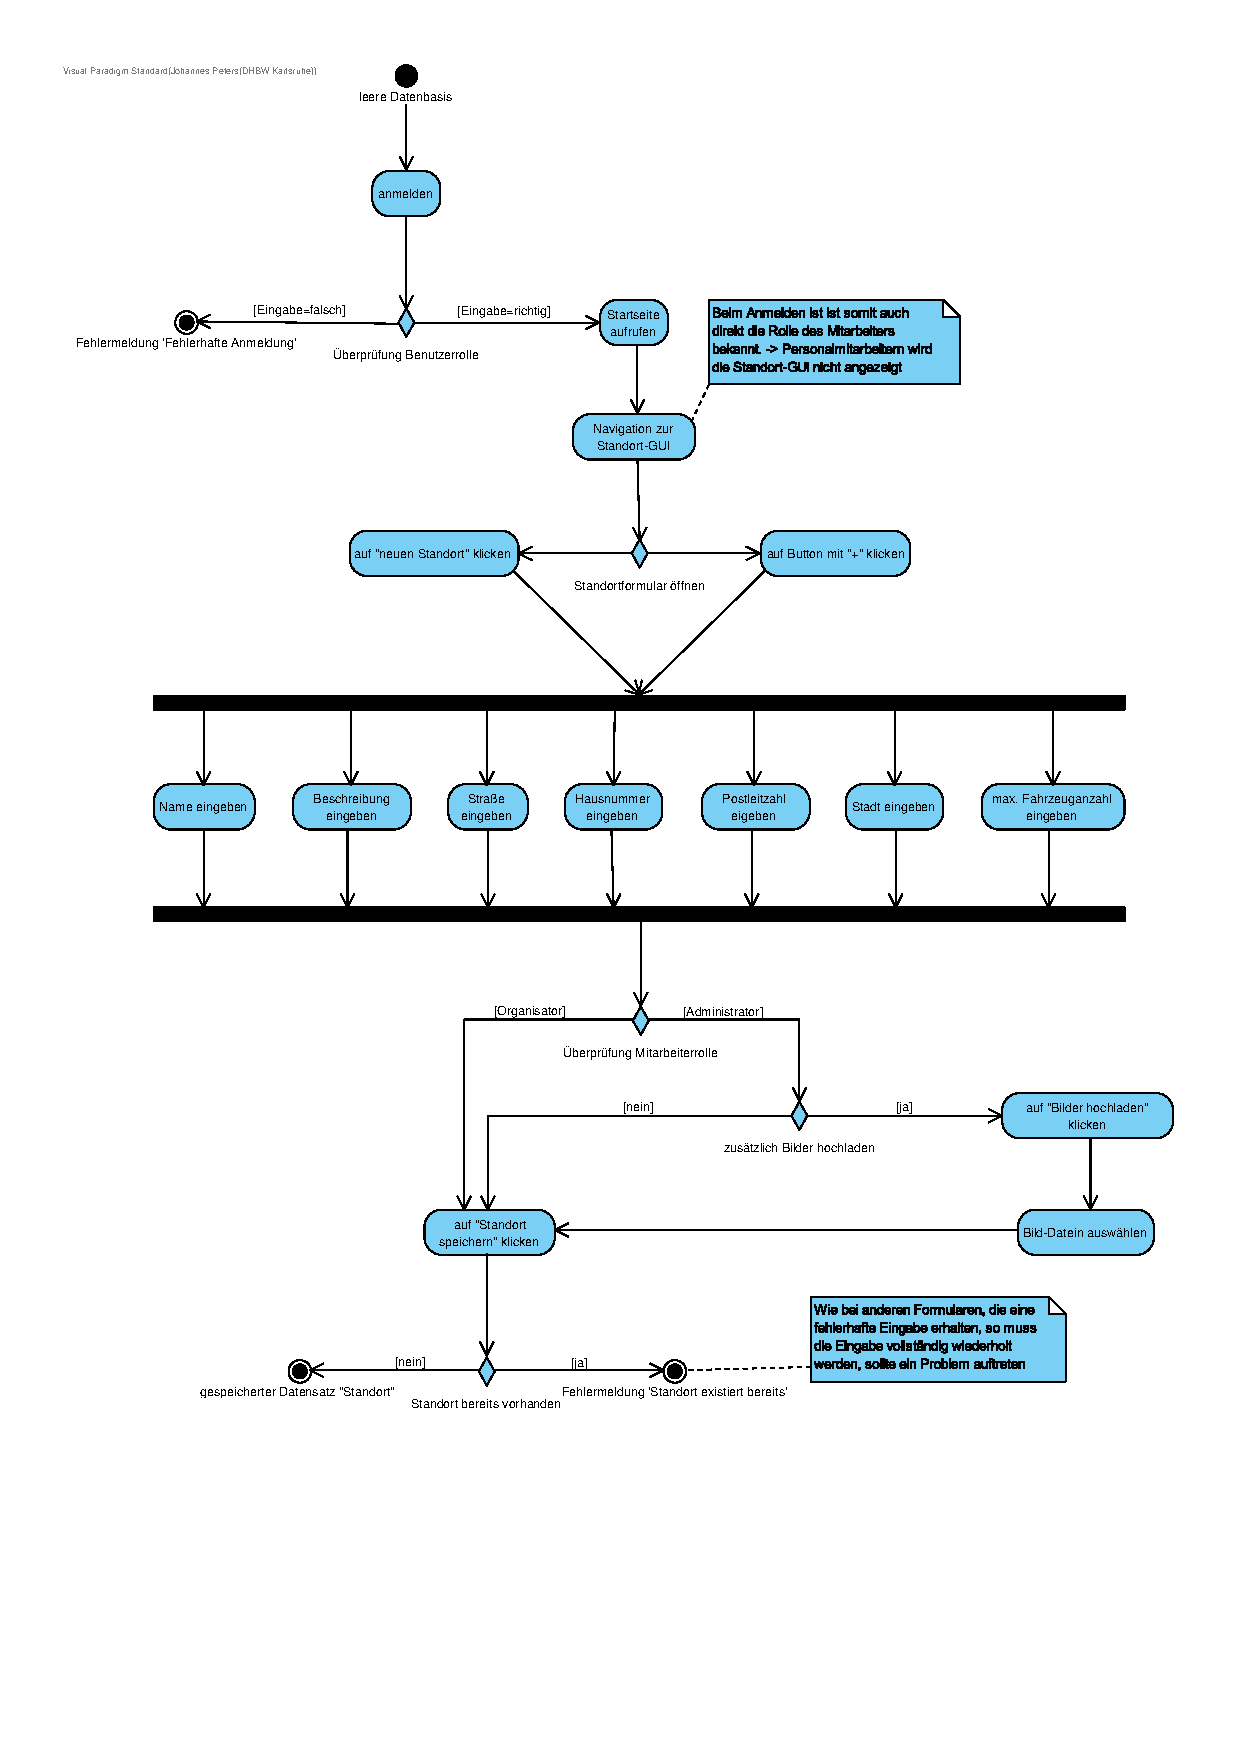
\includegraphics[width=\textwidth, height=\textheight-3cm, trim = 0cm 3cm 0cm 0cm]{Bilder/Diagramme/AD_Standort_anlegen.pdf}
    \caption{Aktivitätsdiagramm: Standort anlegen}
    \label{img:ad_standort}
\end{figure}

Wie bei jeder anderen auf dem System ausgeführten Aktion muss auch beim Anlegen eines neuen Standorts zuerst eine Anmeldung vollzogen werden. Sobald ein Mitarbeiter im System angemeldet ist stehen mittels seines Benutzerprofils auch die Rechte des Nutzers griffbereit. Personalmitarbeiter soll es nicht möglich sein, Standorte anzulegen oder andere Aktionen mit solchen Datensätzen auszuführen, sodass diesen Mitarbeitern eine andere Benutzeroberfläche gezeigt wird wie den Organisatoren und Administratoren. 


Nachdem zu der entsprechenden GUI navigiert wurde und der Mitarbeiter einen neuen Standort anlegen möchte, gibt es zwei Möglichkeiten zum entsprechenden Eingabeformular zu gelangen. Um für die Mitarbeiter, deren IT-Kenntnisse teils mangelhaft sind, mehrere Vorschläge darzustellen gibt es einmal den offensichtlichen Text-Button mit 'neuen Standort anlegen', für die etwas bewanderten Mitarbeiter, zusätzlich einen '+'-Button. Sobald sich das Eingabeformular geöffnet hat, müssen die Felder ausgefüllt werden. 


In welcher Reihenfolge dies ausgeführt wird, ist irrelevant, weshalb im Diagramm diese Aktionen auf parallel dargestellt werden. Sobald alle Texteingaben abgeschlossen wurden, besteht noch die Option Bilder vom Standort hochzuladen, sozusagen ein Titelbild für den Detaileintrag des Standorts. Das Hochladen von Bildern dürfen nur die Administratoren ausführen, sodass zuerst eine Rollenabfrage stattfindet. Sollte ein Administrator diesen Standort anlegen, so wird ihm die Möglichkeit angezeigt und sollte er Bilder hinzufügen möchten, kann er über einen 'Standard-File-Choose-Dialog' Bilder von seinem Computer auswählen und in das Programm laden. Sofern dies erledigt wurde, oder auch nicht, ist es möglich den neuen Standorteintrag zu speichern. 


Bevor der Standort gespeichert wird, erfolgt die Überprüfung, ob dieser Standort bereits vorhanden ist. Sollte das Ergebnis negativ sein, wird der Standort gespeichert. Ist jedoch in der Planung oder Organisation ein Fehler aufgetreten und der Standort exisitiert bereits, erscheint eine Fehlermeldung und die Aktion wird abgebrochen. An sich hätte man im Diagramm anstelle des Endzustandes 'Fehlermeldung' auch eine Schleife einbauen können, die solange läuft wie die Eingabe inkorrekt ist oder bis die Aktion händisch abgebrochen wird. In diesem Fall wird jedoch davon ausgegangen, dass allein auf Basis der Funktionsart eines Eingabeformulars die Eigabefelder geleert werden und die Eingabe wiederholt werden muss. Außer der Abfrage, ob der Standort bereits existiert, findet keine andere logische Überprüfung statt. Sofern sich die Adresse nicht doppelt wird der Datensatz gespeichert. Sollte die Fehlermeldung erscheinen, ist es auch sehr unwahrscheinlich, dass der Mitarbeiter ein zweites Mal die Erstellung des Standortes versucht. 
\newpage

\subsection{Fahrzeug anlegen}

\begin{figure}[!ht]
    \centering
    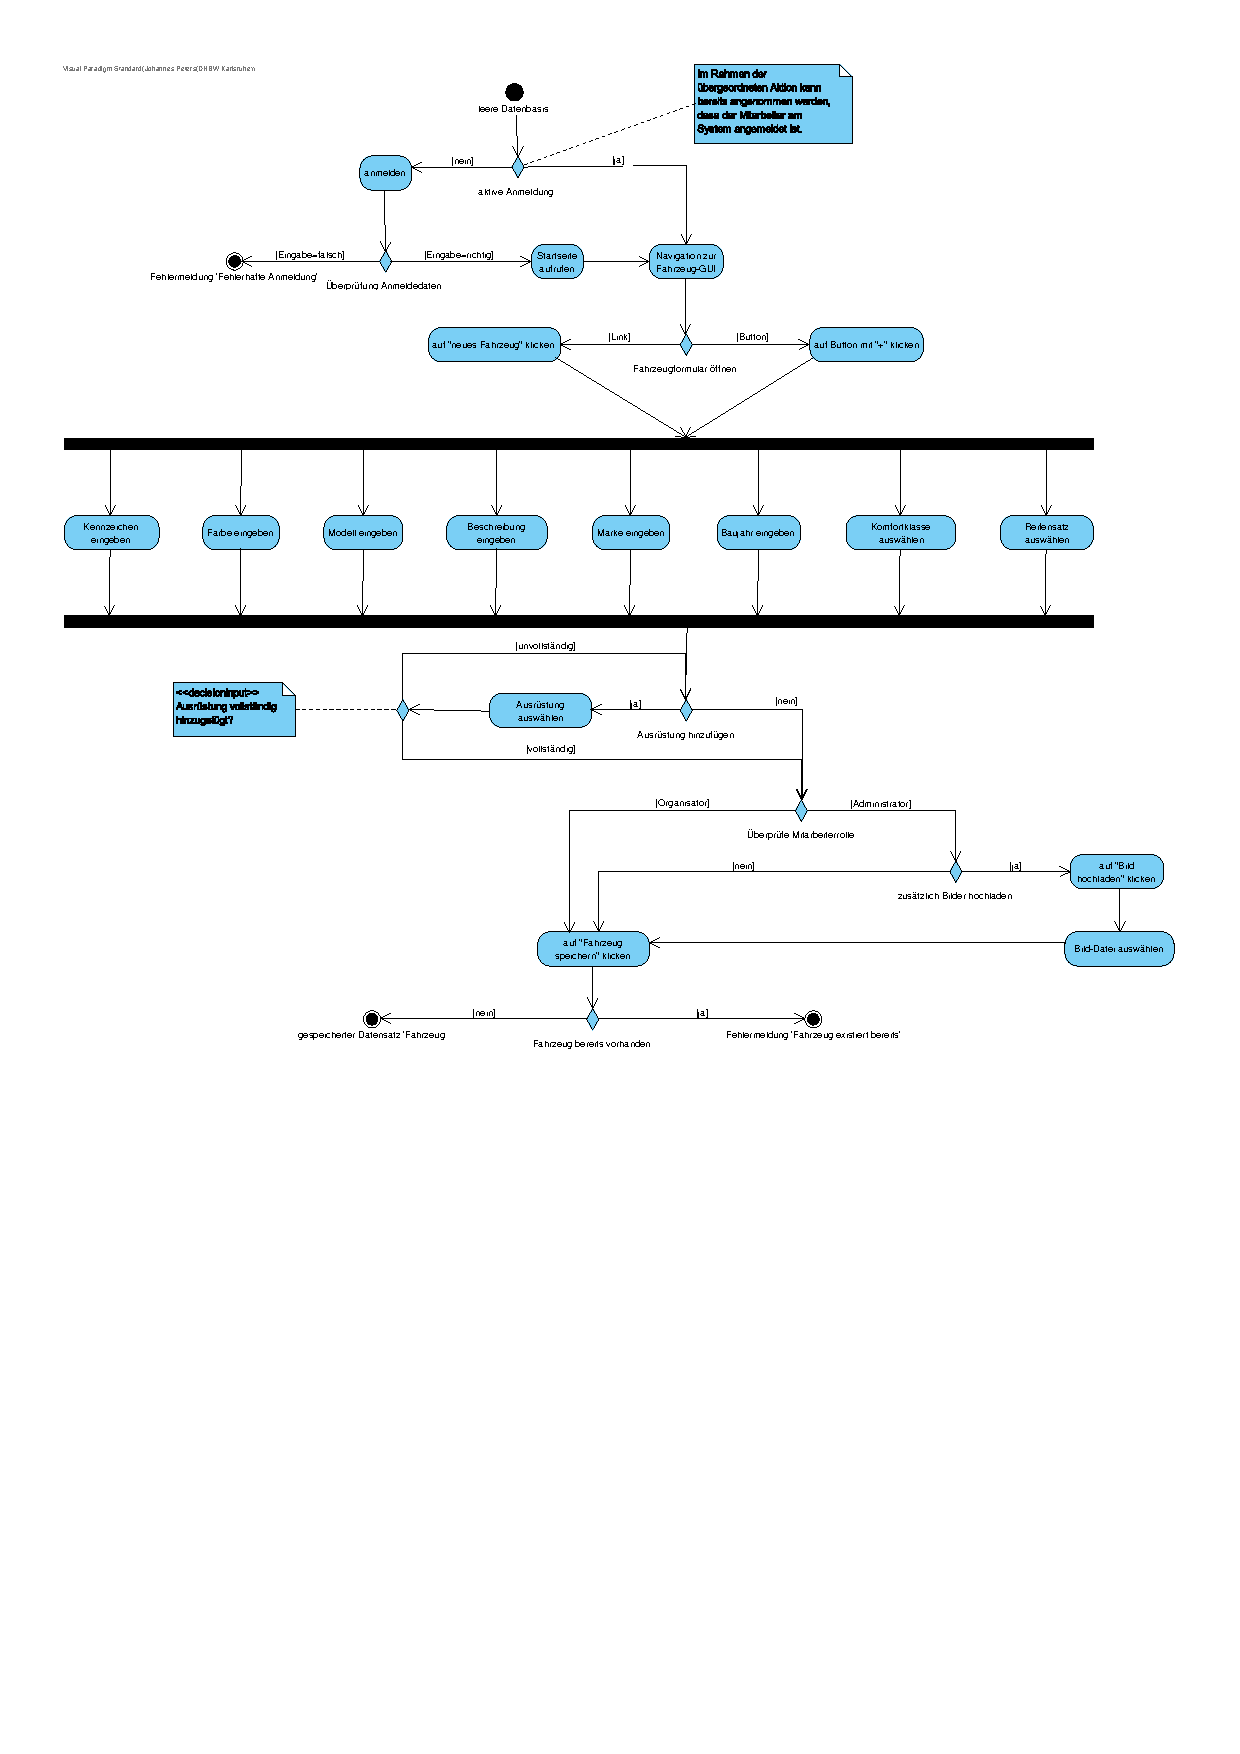
\includegraphics[width=\textwidth, trim = 0cm 11cm 0cm 0cm]{Bilder/Diagramme/AD_Fahrzeug_anlegen.pdf}
    \caption{Aktivitätsdiagramm: Fahrzeug anlegen}
    \label{img:fahrzeug}
\end{figure}

Die eingentliche Aktion, die mit den Aktivitätsdiagrammen analysiert werden soll, ist das Anlegen eines Standortes mit Fahrzeugen. Nur zum besseren Verständnis wurde diese Aktion aufgeteilt, d. h., dass der gesamte Vorgang eigentlich flüssig hintereinander abläuft und der Mitarbeiter, der sich bereits für das Anlegen eines Standortes angemeldet hat, immer noch im System eingeloggt befindet. Theoretisch könnte eine Unterbrechung möglich sein und wurde daher exemplarisch in dieses Diagramm eingebaut. 


Viele Bestandteile des Diagramms sind dem Standort-Diagramm sehr ähnlich, da dass Erstellen und Eingeben von Datensätzen in allen Anwendungsfällen ähnlich ist.


Sollte der Mitarbeiter noch im System tätig sein, so wird er sich bereits irgendwo auf den Benutzeroberflächen befinden und muss sich im Verwaltungsbereich der Anwendung zur Fahrzeug-GUI navigieren. Sollte der Mitarbeiter, aus welchen Gründen auch immer, nicht mehr im System angemeldet sein, so muss dieser sich zuerst wieder anmelden. 


Die Formularbearbeitung ist identisch zum Aufbau bei den Standorten. Da es auch hier irrelevant ist in welcher Reihenfolge die Daten eingegeben werden, wird Parallelisierung verwendet, um dies darzustellen. Die meisten Eingabeaktionen enthalten "eingeben", doch gibt es einige Aktionen, die "auswählen" lauten und somit eine Auswahlmöglichkeit in Form von Drop-Down-Listen implizieren.


Einem Fahrzeug kann Ausrüstung hinzugefügt werden, was durch eine Decision-Node dargestellt wird. Da die Ausrüstung von Fahrzeugen aus Objekten wie Fahrradträger, Dachbox oder Hundetransportskäfig besteht, ist es möglich, dass ein Fahrzeug mehrere Ausrüstungsgegenstände hat. Um eine variable Anzahl an Ausrüstungsgegenständen einem Fahrzeug zuweisen zu können gibt es mittels weiterer Decision-Nodes einen Rückverweis, der solange wiederholt werden kann, bis die hinzugefügte Ausrüstung als vollständig erachtet wird. 


Das Hinzufügen eines Bildes für die Detail-Seite der Fahrzeuge ist bei Fahrzeugen sogar wichtiger als bei einem Standort, aber die Funktionsweise ist trotzdem identisch. Dabei ist das Hinzufügen von Ausrüstungsobjekten und Bildern optional und kann auch später durch Bearbeitung hinzugefügt werden. Bei der Speicherung wird ebenfalls überprüft, ob das Fahrzeug bereits existiert, dabei soll später das Kennzeichen als Vergleichswert verwendet werden. 

\newpage

\subsection{Fahrzeug einem Standort zuordnen}

\begin{figure}[!ht]
    \centering
    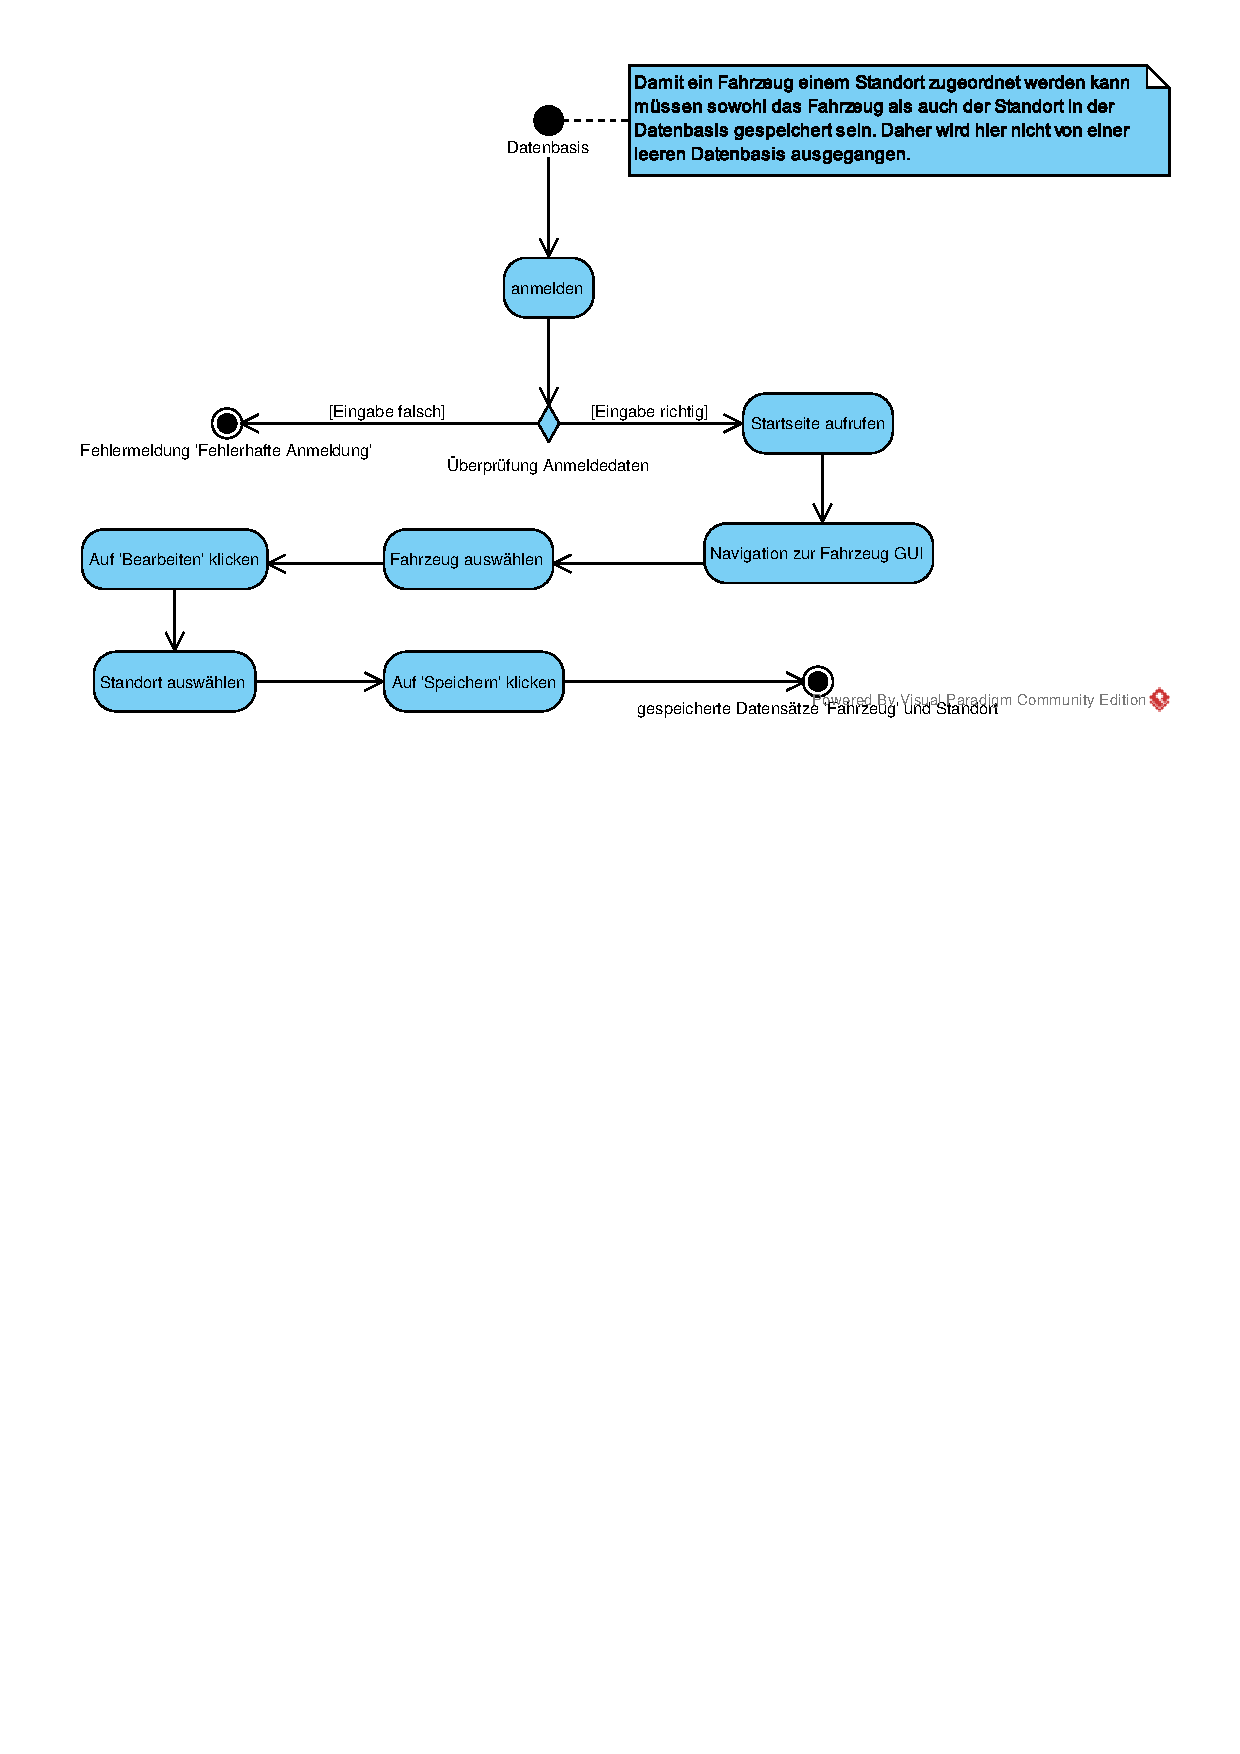
\includegraphics[width=\textwidth, trim = 0cm 11cm 0cm 0cm]{Bilder/Diagramme/FahrzeugStandortZuordnen.pdf}
    \caption{Aktivitätsdiagramm: Fahrzeug einem Standort zuordnen}
    \label{img:fahrzeugzuordnen}
\end{figure}

Nachdem die Standorte und Fahrzeuge angelegt wurden, können die Fahrzeuge einem Standort zugewiesen werden. Die Zuweisung wird in Abbildung \ref{img:fahrzeugzuordnen} dargestellt. Dazu wird davon ausgegangen, dass der Mitarbeiter noch nicht im System angemeldet ist. Daher ist der erste Schritt die Anmeldung im System. Sollte die Eingabe bei der Anmeldung fehlerhaft sein so wird eine Fehlermeldung angezeigt und der Nutzer kann nicht auf die Anwendung zugreifen. Falls die Anmeldung erfolgreich ist, wird dem Nutzer die Startansicht angezeigt. Um nun ein Fahrzeug einem Standort zuzuweisen muss der Nutzer zunächst auf die Fahrzeug-GUI navigieren. Hier kann das Fahrzeug, welches einem Standort zugewiesen werden soll, ausgewählt werden. Nachdem der Nutzer auf 'Bearbeiten geklickt hat, ist die Auswahl eines Standortes möglich. Sobald der Nutzer auf 'Speichern' klickt wird sowohl der Datensatz des Standortes als auch der Datensatz des Fahrzeugs angepasst und gespeichert.

